%%%%%%%%%%%%%%%%%%%%%%%%%%%%%%%%%%%%%%%%%
% Beamer Presentation
% LaTeX Template
% Version 1.0 (10/11/12)
%
% This template has been downloaded from:
% http://www.LaTeXTemplates.com
%
% License:
% CC BY-NC-SA 3.0 (http://creativecommons.org/licenses/by-nc-sa/3.0/)
%
%%%%%%%%%%%%%%%%%%%%%%%%%%%%%%%%%%%%%%%%%

%----------------------------------------------------------------------------------------
%	PACKAGES AND THEMES
%----------------------------------------------------------------------------------------

\documentclass{beamer}

\mode<presentation> {

% The Beamer class comes with a number of default slide themes
% which change the colors and layouts of slides. Below this is a list
% of all the themes, uncomment each in turn to see what they look like.

\usetheme{default}
%\usetheme{AnnArbor}
%\usetheme{Antibes}
%\usetheme{Bergen}
%\usetheme{Berkeley}
%\usetheme{Berlin}
%\usetheme{Boadilla}
%\usetheme{CambridgeUS}
%\usetheme{Copenhagen}
%\usetheme{Darmstadt}
%\usetheme{Dresden}
%\usetheme{Frankfurt}
%\usetheme{Goettingen}
%\usetheme{Hannover}
%\usetheme{Ilmenau}
%\usetheme{JuanLesPins}
%\usetheme{Luebeck}
%\usetheme{Madrid}
%\usetheme{Malmoe}
%\usetheme{Marburg}
%\usetheme{Montpellier}
%\usetheme{PaloAlto}
%\usetheme{Pittsburgh}
%\usetheme{Rochester}
%\usetheme{Singapore}
%\usetheme{Szeged}
%\usetheme{Warsaw}

% As well as themes, the Beamer class has a number of color themes
% for any slide theme. Uncomment each of these, in turn, to see how it
% changes the colors of your current slide theme.

%\usecolortheme{albatross}
%\usecolortheme{beaver}
%\usecolortheme{beetle}
%\usecolortheme{crane}
%\usecolortheme{dolphin}
\usecolortheme{dove}
%\usecolortheme{fly}
%\usecolortheme{lily}
%\usecolortheme{orchid}
%\usecolortheme{rose}
%\usecolortheme{seagull}
%\usecolortheme{seahorse}
%\usecolortheme{whale}
%\usecolortheme{wolverine}

%\setbeamertemplate{footline} % To remove the footer line in all slides uncomment this line
%\setbeamertemplate{footline}[page number] % To replace the footer line in all slides with a simple slide count uncomment this line

%\setbeamertemplate{navigation symbols}{} % To remove the navigation symbols from the bottom of all slides, uncomment this line
}
\usepackage{fontspec}
\usepackage{bibentry}
\usepackage{graphicx} % Allows including images
\usepackage{booktabs} % Allows the use of \toprule, \midrule and \bottomrule in tables

\setmainfont{ArialMT}
%\setbeamertemplate{frametitle}[default][center]

%----------------------------------------------------------------------------------------
%	TITLE PAGE
%----------------------------------------------------------------------------------------

\title[Exercise Recommendation]{Research on High School Math Exercise Recommendation Based on Graph Neural Network} % The short title appears at the bottom of every slide; the full title is only on the title page

\author{Wangzhihui Mei} % Your name
\institute[UOW] 
{
University of Wollongong \\ % Your institution for the title page
\medskip
\textit{maywzh@gmail.com} % Your email address
}
\date{\today} % Date, can be changed to a custom date

\begin{document}

\begin{frame}
  \titlepage % Print the title page as the first slide
\end{frame}

\begin{frame}
  \frametitle{Overview} % Table of contents slide, comment this block out to remove it
  \tableofcontents % Throughout your presentation, if you choose to use \section{} and \subsection{} commands, these will automatically be printed on this slide as an overview of your presentation
\end{frame}

%----------------------------------------------------------------------------------------
%	PRESENTATION SLIDES
%----------------------------------------------------------------------------------------

%------------------------------------------------
\section{Introduction} % Sections can be created in order to organize your presentation into discrete blocks, all sections and subsecti ons are automatically printed in the table of contents as an overview of the talk
%------------------------------------------------

\subsection{Research Topic}
\begin{frame}
  \frametitle{Background}
  \begin{itemize}
    \item Knowledge State Monitoring
    \item Learning Resource Recommendation
    \item High School Math
  \end{itemize}
\end{frame}

%------------------------------------------------
\begin{frame}
  \frametitle{Problems}
  \begin{itemize}
    \item Disorganized exercise corpus lacking knowledge tags
    \item Hard to evaluate the knowledge mastery status
    \item Difficult to find appropriate exercise for improving knowledge mastery
  \end{itemize}
\end{frame}
%------------------------------------------------
\begin{frame}
  \frametitle{Core of Research}
  \begin{block}{Exercise Labelling}

  \end{block}
  \begin{block}{}
    Hard to evaluate the knowledge mastery status
  \end{block}
  \begin{block}{}
    Difficult to find appropriate exercise for improving knowledge mastery
  \end{block}
  \begin{alertblock}{aaaa}
    sdfsdfsad
  \end{alertblock}
\end{frame}
%------------------------------------------------
\subsection{Research Content}
\begin{frame}
  \frametitle{Knowledge Tagging}
  \begin{figure}
    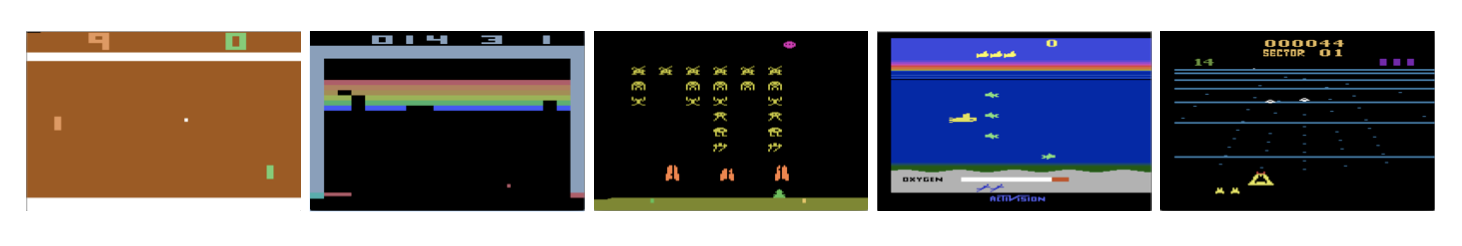
\includegraphics[width=1.0\textwidth]{figures/atari.png}
  \end{figure}
\end{frame}

%------------------------------------------------

\begin{frame}
  \frametitle{Knowledge Tracing}

\end{frame}

%------------------------------------------------

\begin{frame}
  \frametitle{Exercise Recommendation}
  \begin{block}{Block 1}
    content
  \end{block}

  \begin{block}{Block 2}
    content
  \end{block}

  \begin{block}{Block 3}
    content
  \end{block}
\end{frame}

%------------------------------------------------
\section{Proposed Model}
%------------------------------------------------
\begin{frame}
  \
\end{frame}




\begin{frame}
  \frametitle{Exercise Knowledge Tagging}
  \begin{columns}[c] % The "c" option specifies centered vertical alignment while the "t" option is used for top vertical alignment

    \column{.45\textwidth} % Left column and width
    \textbf{Heading}
    \begin{enumerate}
      \item Statement
      \item Explanation
      \item Example Table~\ref{tbl:t1}
    \end{enumerate}

    \column{.5\textwidth} % Right column and width


  \end{columns}
\end{frame}

%------------------------------------------------
\begin{frame}
  \frametitle{Table}
  \begin{table}
    \caption{Table caption}\label{tbl:t1}
    \begin{tabular}{l l l}
      \toprule
      \textbf{Treatments} & \textbf{Response 1} & \textbf{Response 2} \\
      \midrule
      Treatment 1         & 0.0003262           & 0.562               \\
      Treatment 2         & 0.0015681           & 0.910               \\
      Treatment 3         & 0.0009271           & 0.296               \\
      \bottomrule
    \end{tabular}
  \end{table}
\end{frame}

%------------------------------------------------

\begin{frame}
  \frametitle{Theorem}
  \begin{theorem}[Mass-energy equivalence]
    \(E = mc^2\)
  \end{theorem}
\end{frame}

%------------------------------------------------

\begin{frame}[fragile] % Need to use the fragile option when verbatim is used in the slide
  \frametitle{Verbatim}
  \begin{example}[Theorem Slide Code]
    \begin{verbatim}
\begin{frame}
\frametitle{Theorem}
\begin{theorem}[Mass--energy equivalence]
$E = mc^2$
\end{theorem}
\end{frame}\end{verbatim}
  \end{example}
\end{frame}

%------------------------------------------------
\section{Result}
\begin{frame}
  \frametitle{Figure}
  Uncomment the code on this slide to include your own image from the same directory as the template .TeX file.
  %\begin{figure}
  %\includegraphics[width=0.8\linewidth]{test}
  %\end{figure}
\end{frame}

%------------------------------------------------

\begin{frame}[fragile] % Need to use the fragile option when verbatim is used in the slide
  \frametitle{Citation}
  An example of the \verb|\cite| command to cite within the presentation:\\~

  This statement requires citation~\cite{shamir2010learning}.
\end{frame}

%------------------------------------------------

% \begin{frame}
%     \frametitle{References}
%     \footnotesize{
%         \begin{thebibliography}{99} % Beamer does not support BibTeX so references must be inserted manually as below
%             \bibitem[Smith, 2012]{p1} John Smith (2012)
%             \newblock Title of the publication
%             \newblock \emph{Journal Name} 12(3), 45 -- 678.
%         \end{thebibliography}
%     }
% \end{frame}

\begin{frame}[allowframebreaks]{References}
  %\bibliographystyle{plain}
  \bibliographystyle{amsalpha}
  %\bibliography{mybeamer} also works
  \bibliography{./ref.bib}
\end{frame}

%------------------------------------------------

\begin{frame}
  \Huge{\centerline{The End}}
\end{frame}

%----------------------------------------------------------------------------------------

\end{document}